To calculate the expected separation between the SM Higgs and other 
exotic resonances, we use the same number of events for the exotic resonance
after the full selections as in the SM Higgs case. The expected yields from the 
associated Higgs production, together with the vector boson 
fusion production, remain untouched assuming their SM values. These models 
are comparing different $gg \to H$ production mechanisms.

Figure~\ref{fig:expsep2} shows the distributions of 
$q=-2\text{ln}({\cal L}_{2_\text{min}^+}/{\cal L}_{\text{0}^+})$
with generated samples of background and signal of the SM Higgs and 
$2_\text{min}^+$ Graviton at 125 $\GeV$. 
The yields used in the generation of the pseudo-experiments are those 
expected with the full 7+8 $\TeV$ dataset. 
The mean of the expected SM $0^+$ distribution is 1.9 standard deviations 
in the tail of the $2_\text{min}^+$ distribution, while 
the mean of the expected $2_\text{min}^+$ distribution is 2.4 standard deviations 
in the tail of the $0^+$ distribution. The average separation between the two 
hypotheses is about $2.2\sigma$.

%%%%%%%%%%%%%%%%%%%%%%%%%%%%%%%%%%%%%%%%%%%%%
\begin{figure}[!hbtp]
\centering
\label{subfig:res}
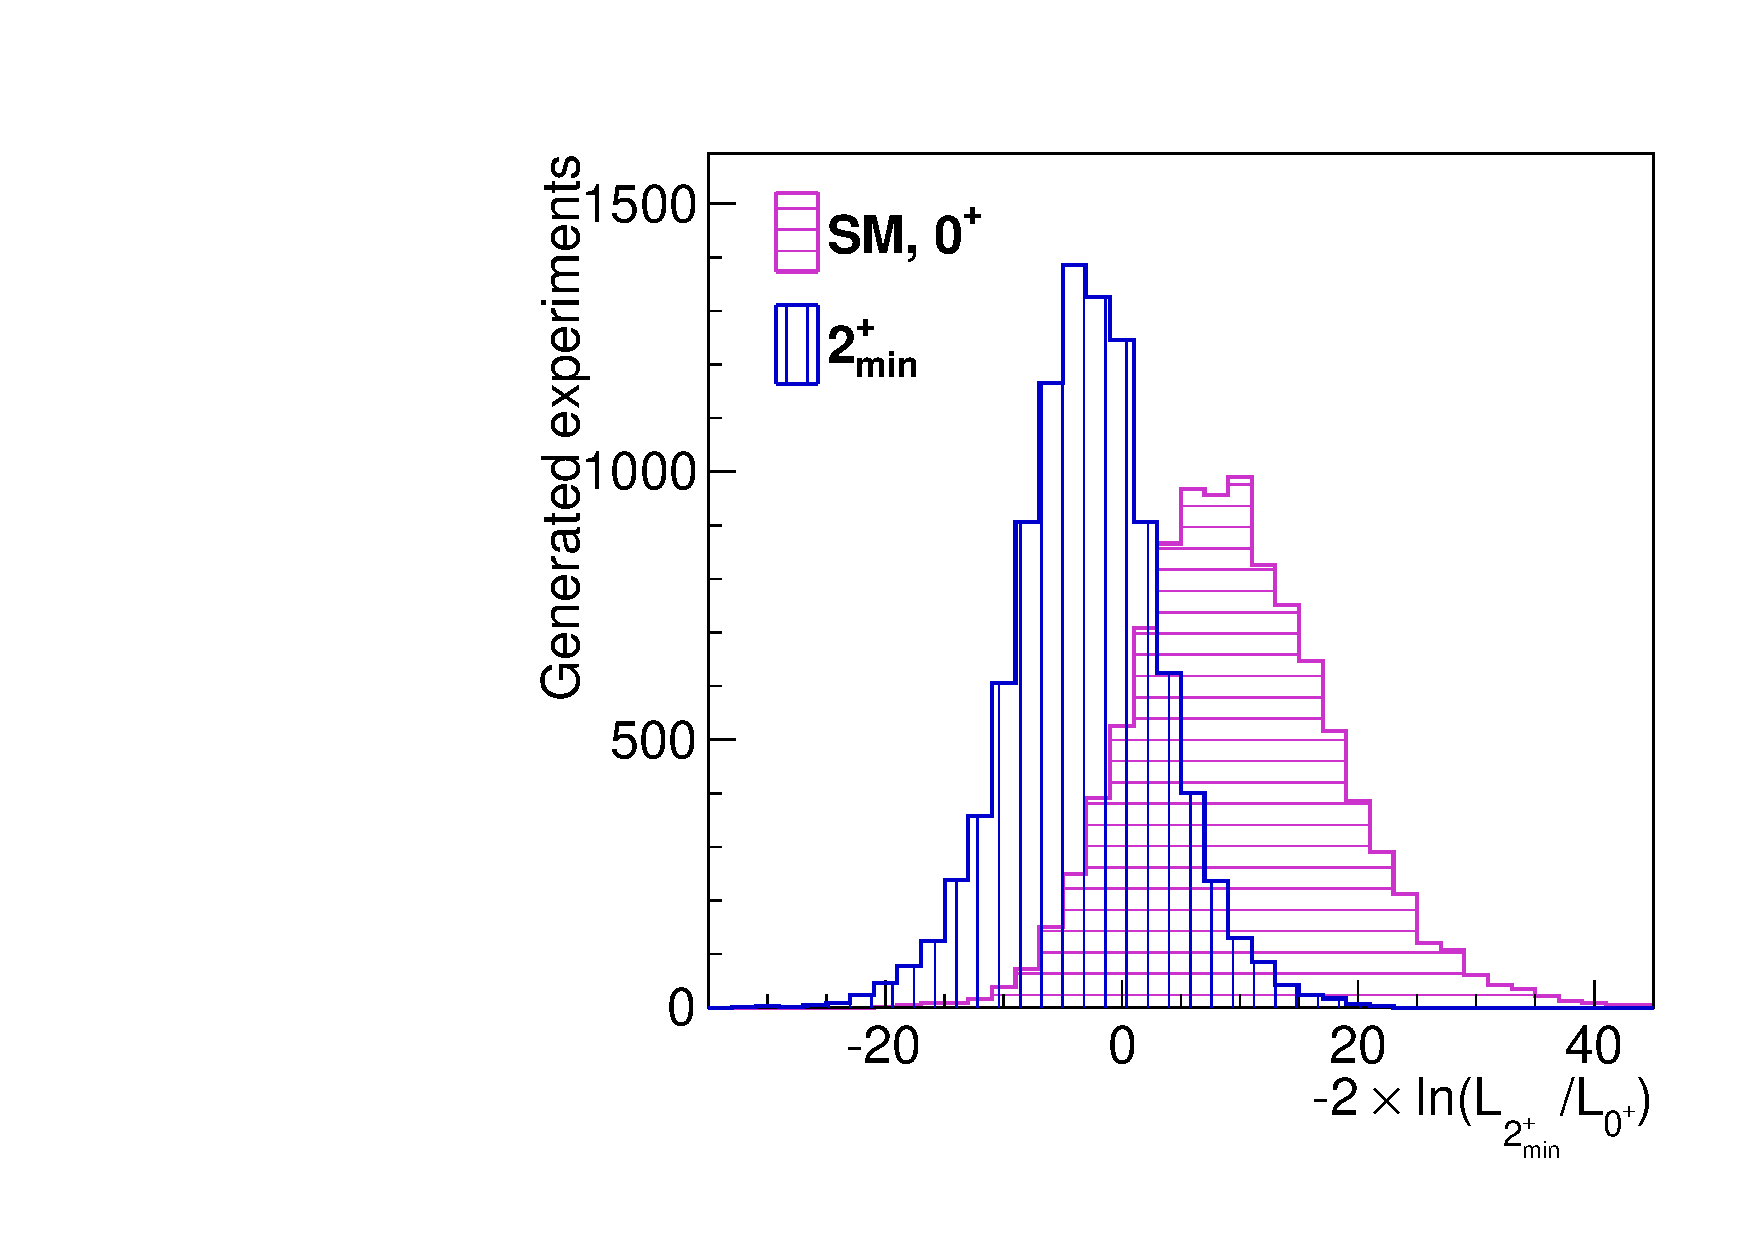
\includegraphics[width=.7\textwidth]{figures/hypo_separation.pdf}
\caption{Distributions of 
$q=-2\text{ln}({\cal L}_{2_\text{min}^+}/{\cal L}_{\text{0}^+})$ 
of pseudo-experiments according to two signal types, $0^+$ (horizontally hatched histogram) 
and $2_\text{min}^+$ (vertically hatched histogram) at $\mHi = 125~\GeV$. 
The yields used in the generation of the pseudo-experiments are those 
expected with the full 7+8 $\TeV$. 
}
\label{fig:expsep2}
\end{figure}
%%%%%%%%%%%%%%%%%%%%%%%%%%%%%%%%%%%%%%%%%%%%%

The same study is performed to compare $0^+$ (SM prediction) and 
$0^-$ hypotheses. Figure~\ref{fig:expsep0} shows the distributions of 
$q=-2\text{ln}({\cal L}_{0^-}/{\cal L}_{\text{0}^+})$. 
The mean of the expected SM $0^+$ distribution is 0.9 standard deviations 
in the tail of the $0^-$ distribution, while 
the mean of the expected $0^-$ distribution is 1.1 standard deviations 
in the tail of the $0^+$ distribution. The average separation between the two 
hypotheses is about $1.0\sigma$. The expected separation in this 
case is small since the two processes are rather similar in 
the studied final state topology.

%%%%%%%%%%%%%%%%%%%%%%%%%%%%%%%%%%%%%%%%%%%%%
\begin{figure}[!hbtp]
\centering
\label{subfig:res}
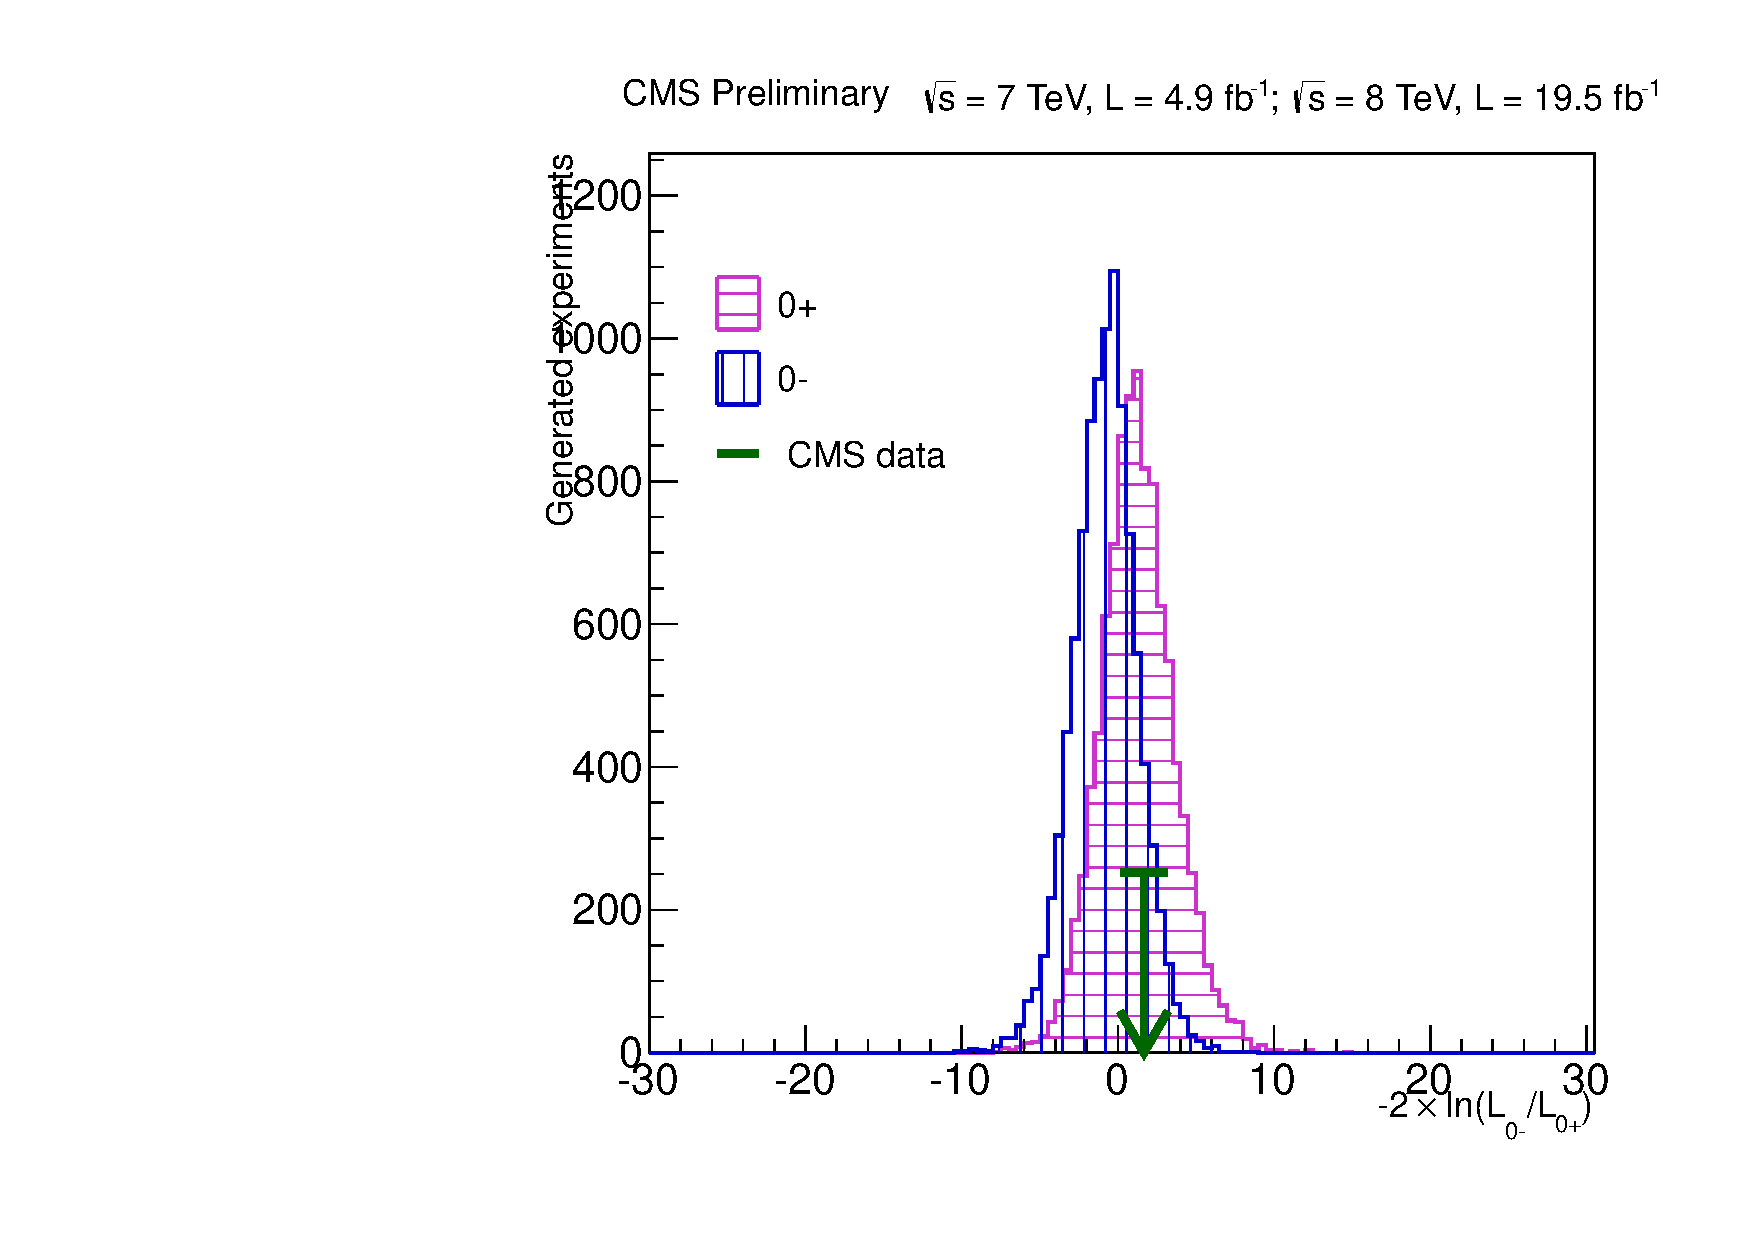
\includegraphics[width=.7\textwidth]{figures/sigsep_combine_0.pdf}
\caption{Distributions of 
$q=-2\text{ln}({\cal L}_{0_\text{min}^-}/{\cal L}_{\text{0}^+})$ 
of pseudo-experiments according to two signal types, $0^+$ (horizontally hatched histogram) 
and $0^-$ (vertically hatched histogram) at $\mHi = 125~\GeV$. 
The yields used in the generation of the pseudo-experiments are those 
expected with the full 7+8 $\TeV$. 
}
\label{fig:expsep0}
\end{figure}
%%%%%%%%%%%%%%%%%%%%%%%%%%%%%%%%%%%%%%%%%%%%%
